% -*- coding: utf-8; -*-

\chapter{Plano de Ação}
\label{cha:Plano de Ação}

Para modelar o sistema, foi realizada uma validação do problema. Alunos do departamento de informática da universidade foram entrevistados afim de descobrir quais dificuldades enfrentam durante o processo de matrícula e quais são as suas preferências ao montar uma grade disciplinar. O objetivo era identificar quais características de uma grade disciplinar contribuem para a satisfação do aluno e adicionar as funcionalidades necessárias no sistema e no algoritmo.

Com o problema validado, então o projeto passou por uma etapa de pesquisa. 
Foram estudados diferentes algoritmos de recomendação em contextos semelhantes ao sistema a ser desenvolvido, afim de se projetar o algoritmo que mais se adequa às necessidades do problema validado. 
Nessa etapa, também foram analisadas as fontes de informações disponibilizadas pela universidade e como cada fonte pode ser integrada no sistema. 
Por exemplo, já existia uma biblioteca\footnote{Dispon\'ivel em: \url{https://pypi.org/project/microhorario-dl/}} Python para acessar e processar as disciplinas atualmente no microhorario.

Após a etapa de pesquisa, o algoritmo começou a ser desenvolvido. 
Depois de obter um algoritmo minimamente viável, foi desenvolvida a interface de planejamento para mostrar o funcionamento do algoritmo. 
Tanto o algoritmo com a interface foram desenvolvidas utilizando um modelo de desenvolvimento incremental, para que o sistema passe por etapas de desenvolvimento, teste e validação com os alunos. 

\section{Cronograma original}

O cronograma inicial pode ser visualizado na figura \ref{fig-cronograma}.

\begin{figure}[ht!]
    \begin{center}
    
\includegraphics[width=260pt]{figuras/cronograma}
    \caption{Cronograma original do projeto}
    \label{fig-cronograma}
    \end{center}
\end{figure}

\section{Cronograma revisado}

% TODO: revisar o cronograma

==== A SER MODIFICADO ====

O plano de ação original foi levemente modificado. A validação do problema durou um pouco mais do que planejado. As etapas relacionadas ao algoritmo foram agrupadas no desenvolvimento do sistema, e foi criada uma nova etapa de elaboração de requisitos. O cronograma revisado pode ser visualizado na figura \ref{fig-cronograma-atualizado}.

\begin{figure}[ht!]
    \begin{center}
    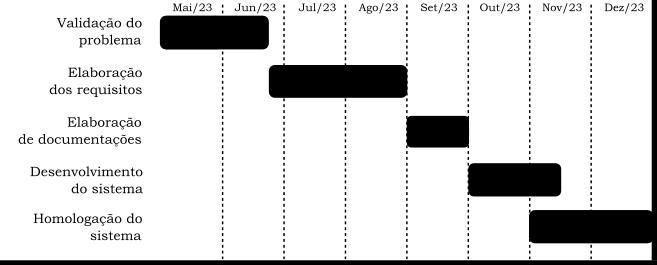
\includegraphics[width=260pt]{figuras/cronograma-atualizado}
    \caption{Cronograma atualizado do projeto}
    \label{fig-cronograma-atualizado}
    \end{center}
\end{figure}